%% Ankur Sinha

%% packages %%
% support for coloured text
\usepackage{color}
% IPA
\usepackage{tipa}
\usepackage[scale=2]{ccicons}
\usepackage{amssymb}
\usepackage{tikz}
\usetikzlibrary{mindmap, arrows.meta, positioning, arrows}
\usepackage{pgfplots}
% Define the colours we use for E and I in all graphs
\usepackage{jneurosci}
\usepackage{subcaption}
\usepackage[T1]{fontenc}
\usepackage[utf8]{inputenc}
% \usepackage[style=nature,backend=biber,autocite=footnote]{biblatex}
% \addbibresource{/home/asinha/Documents/01_Readables/00_research_papers/bibliography/masterbib.bib}
% \renewcommand*{\bibfont}{\tiny}
% Use opensans
% \usepackage[default,scale=0.95]{opensans}
\usepackage[sfdefault]{roboto}
% for strike through
\usepackage[normalem]{ulem}
% links, urls, refs
\definecolor{links}{HTML}{2A1B81}
% Fedora blue for the theme
\definecolor{FedoraBlue}{HTML}{2A1B81}
\usepackage{hyperref}
\hypersetup{colorlinks,linkcolor=Green,urlcolor=links}
% graphics
\usepackage{graphicx}
% algorithm
\usepackage{algorithmic}
\usepackage{textcomp}
\usepackage{wrapfig}
\usepackage{textgreek}
\usepackage{euler}
\usepackage{tabularx}
\usepackage{booktabs}
\usepackage{minted}
\usepackage{csquotes}
% beamer theme
% use defaults for theme
\usetheme[numbering=fraction]{metropolis}
\usefonttheme[onlymath]{serif}
\setbeamerfont{footnote}{size=\tiny}
\setbeamerfont{caption}{size=\tiny}
\setbeamercolor{alerted text}{fg=Green}
\setbeamerfont{note page}{size=\small}

% Not needed in metropolis, but in general footnote citation fixes: https://tex.stackexchange.com/questions/44217/how-can-i-stop-footcite-from-hijacking-my-beamer-columns
% how to use multiple references to the same footnote: https://tex.stackexchange.com/questions/27763/beamer-multiple-references-to-the-same-footnote

% Disable footnoterule
\renewcommand{\footnoterule}{}

%% title %%
\title{Docs for public software projects}
\author[Ankur Sinha]{Ankur Sinha}
\date{29/10/2020}

%% document begins %%
\begin{document}


% title frame %%
\begin{frame}
  \titlepage{}
\end{frame}
%% Three slides for 5 minutes seems good
%% So, 30 slides at most for 50 minutes
\section{Documentation?}
\begin{frame}[c]
  \frametitle{Docs for different target audiences: dev docs}
  \begin{itemize}
    \item In-source comments: help to understand the source code,
    \item Change log: what changed and when (version control).
    \item Standard Operating Procedures (SOPs): ensure no single point of contact/failure (SPOC/F):
      \begin{itemize}
        \item API/ABI versioning and software release SOP,
        \item Continuous integration (CI) SOP,
        \item Deployment SOP,
        \item Contribution guidelines: pull request workflow etc.
      \end{itemize}
  \end{itemize}
\end{frame}
\begin{frame}[fragile]
  \frametitle{Dev docs are conversations between devs}
  \begin{minted}{cpp}
 /*
 * Dear Maintainer
 *
 * Once you are done trying to 'optimize' this routine,
 * and you have realized what a terrible mistake that was,
 * please increment the following counter as a warning
 * to the next guy.
 *
 * total_hours_wasted_here = 73
 */
  \end{minted}
  \footnotetext[1]{\href{https://loudprogrammer.net/best-comments-in-source-code-i-ever-encountered/}{Top 45 Best Comments In Source Code I Ever Encountered}}
\end{frame}
% \begin{frame}[fragile]
  % \frametitle{Change logs/commit logs: not for users either}
  % \begin{figure}[h]
    % \centering
    % 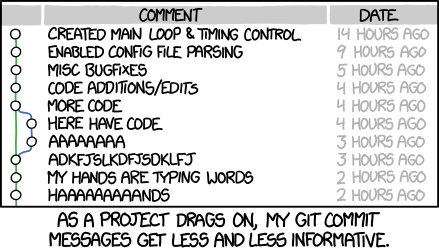
\includegraphics[width=0.8\linewidth]{99_images/git_commit}
  % \end{figure}
  % \footnotetext[2]{\href{ https://xkcd.com/1296/  }{ xkcd: Git Commit  }}
  % \footnotetext[3]{\href{ https://chris.beams.io/posts/git-commit/  }{ How to Write a Git Commit Message  }}
% \end{frame}
\begin{frame}[c]
  \frametitle{Docs for different target audiences: user docs}
  \begin{itemize}
    \item Tools: how to \alert{use} the tool, options, features, extensions \ldots{}
    \item Libraries: how to \alert{use} the API,
    \item Example code snippets, guides.
  \end{itemize}
\end{frame}
\begin{frame}[c]
  \frametitle{Docs for users: separate from development}
  \begin{itemize}
    \item \textbf{Must} clearly define what the tool (software) does,
    \item \textbf{Must} define \alert{entry-points} for users to get started with the software,
    \item \textbf{Must} provide a \alert{high level} overview of concepts needed to use the software,
    \item \textbf{Should} provide references to detailed definitions of these concepts,
    \item \textbf{Must} list channels of communication etc.\ for users,
      \pause{}
    \item \textbf{May} be generated from comments in the source code but \textbf{must not} be written like developer documentation.
  \end{itemize}
\end{frame}
\begin{frame}[c]
  \frametitle{Case study: NeuroML}
  \href{https://neuroml.org}{neuroml.org}
\end{frame}
\section{Publishing docs: software}
\begin{frame}[c]
  \frametitle{Documentation tools: translators}
  Docs sources \(\rightarrow\) documentation tool \(\rightarrow\) HTML/PDF/\ldots{}\\
  Today: \alert{Sphinx}, \alert{Jupyter-book}.
\end{frame}
\begin{frame}[c]
  \frametitle{Sphinx: Python default}
  \begin{itemize}
    \item Inputs sources:
      \begin{itemize}
        \item reStructuredText (default),
        \item Markdown (CommonMark \emph{flavour}\footnotemark[3]{})
        \item MyST (Markdown + reStructuredText)\footnotemark[4]{}
      \end{itemize}
    \item Output formats:
      \begin{itemize}
        \item HTML (multi-page and single-page),
        \item \LaTeX{} for PDFs, ePub, Texinfo, Man pages, \ldots{}
      \end{itemize}
  \end{itemize}
  \footnotetext[2]{\href{ https://www.sphinx-doc.org/en/master/  }{ Overview --- Sphinx 4.0.0+ documentation  }}
  \footnotetext[3]{The original Markdown specification is not unambiguous, and so multiple flavours of Markdown have cropped up over the years. CommonMark is one attempt at standardisation. GitHub Flavoured Markdown is another that GitHub created.}
  \footnotetext[4]{\href{ https://myst-parser.readthedocs.io/en/latest/  }{ MyST - Markedly Structured Text  }}
\end{frame}
\begin{frame}[c]
  \frametitle{Sphinx examples}
  Demo!
\end{frame}
\begin{frame}[c]
  \frametitle{Jupyter-book: shiny new Jupyter based system}
  \begin{itemize}
    \item Input sources:
      \begin{itemize}
        \item Jupyter Markdown,
        \item Jupyter notebooks: Python, Julia, Ruby, Haskell \ldots{},
        \item MyST,
        \item reStructuredText.
      \end{itemize}
    \item Output formats:
      \begin{itemize}
        \item HTML (multi-page and single-page),
        \item PDF\@.
      \end{itemize}
    \item \alert{Interactive pages!}
      \begin{itemize}
        \item Binder, JupyterHub, Google Colab, ThebeLab\footnotemark[6]{}.
      \end{itemize}
      \footnotetext[5]{\href{ https://jupyterbook.org/intro.html  }{ Books with Jupyter  }}
      \footnotetext[6]{Embedded: so no need to leave the page.}
  \end{itemize}
\end{frame}
\begin{frame}[c]
  \frametitle{Jupyter-book example: NeuroML documentation}
  Demo!
\end{frame}
\begin{frame}[c]
  \frametitle{Lab website updates?}
  \href{www.silverlab.org}{www.silverlab.org}
\end{frame}
\end{document}
